\documentclass[tikz,border=0pt]{standalone}
\usepackage[utf8]{inputenc}
\usepackage{csquotes}
\usepackage{xcolor}
\usepackage{graphicx}
\usepackage{pgffor}
\usepackage{listings}
\usepackage{array}
\usepackage{fontawesome}
\usepackage{amsmath}

\lstset{
    basicstyle=\ttfamily\fontsize{16}{18}\selectfont,
    breaklines=true,
    % backgroundcolor=\color{black},
    keywordstyle=\color{pink},
    commentstyle=\color{blue},
    stringstyle=\color{white},
    showstringspaces=false,
    frame=none,
    xleftmargin=0.6cm,
    xrightmargin=0.6cm
}

\begin{document}
\begin{tikzpicture}
\useasboundingbox (0,0) rectangle (10.8,10.8);

% Hintergrund in Schwarz
\fill[black] (0,0) rectangle (10.8,10.8);

% Zufällige Einsen und Nullen verteilen
\foreach \i in {1,...,5000} {
    \node[text=green, opacity=0.1, font=\ttfamily\fontsize{5}{6}\selectfont] at (rand*10.8, rand*10.8) {\pgfmathtruncatemacro{\random}{round(rand)}\random};
}

% \fill[red, opacity=0.1] (0.05,5.95) rectangle (10.75,10.75);
% \draw[red, thin] (0.05,5.95) rectangle (10.75,10.75); % 45% Höhe
% \node[red, anchor=north west, font=\ttfamily\bfseries\fontsize{8}{9}\selectfont] at (0.1,10.65) {Problem:};
% % ------------------------------------------------------------------------------------------------------------------------------
% \node[red, anchor=north west, font=\ttfamily\fontsize{8}{9}\selectfont, text width=10.6cm, align=center] at (0.1,10.25) {
% \newline
% \newline
% \newline
% If you want to succeed in penetration testing and cybersecurity, learn at least:
% \newline
% };
% ------------------------------------------------------------------------------------------------------------------------------
\fill[green, opacity=0.1] (0.05,1.15) rectangle (10.75,10.75);
\draw[green, thin] (0.05,1.15) rectangle (10.75,10.75); % 45% Höhe
% \node[green, anchor=north west, font=\ttfamily\bfseries\fontsize{8}{9}\selectfont] at (0.1,5.65) {Solution:};
% ------------------------------------------------------------------------------------------------------------------------------
\node[green, anchor=north west, font=\ttfamily\fontsize{8}{9}\selectfont, text width=10.6cm, align=center] at (0.1,10.25) {
    \begin{quote}
        23. November was Fibonacci Day, which is defined mathematically as:
        {\small 
        \begin{equation}
            F(n) = 
            \begin{cases} 
                0, & \text{if } n = 0 \\ 
                1, & \text{if } n = 1 \\ 
                F(n-1) + F(n-2), & \text{if } n > 1
            \end{cases}
        \end{equation}
        
        % \textbf{Explanation of variables:}
        % \begin{itemize}
        %     \item $F(n)$: The Fibonacci number at position $n$.
        %     \item $n$: The position in the Fibonacci sequence (starting from 0).
        %     \item $F(n-1)$: The previous Fibonacci number.
        %     \item $F(n-2)$: The second previous Fibonacci number.
        % \end{itemize}
        }
        
        \vspace{2em} % Funktioniert für den Abstand zum Autor
        
        \hfill -- {\small \textit{"Leonardo von Pisa (Fibonacci)"}}
        \end{quote}        
\vspace{3em}
Fibonacci numbers possible in:\\
\begin{itemize}
    \item Key generation
    \item Random number generation
    \item Network-DoS attack detection
    \item Better "Hello World" for each programming language
\end{itemize}
};
% ------------------------------------------------------------------------------------------------------------------------------
\draw[green, thin] (0.05,0.05) rectangle (10.75,1.05); % 10% Höhe
% \node[green, anchor=north west, font=\ttfamily\bfseries\fontsize{5}{6}\selectfont] at (0.1,0.95) {Contact:};

% Tabelle 2x2 im Contact Block
\node[green, anchor=north west, font=\ttfamily\fontsize{8}{9}\selectfont, text width=10.6cm] at (0.1,0.95) {
\begin{tabular}{@{}p{4.8cm}@{}p{5cm}@{}}
\faGlobe\ https://cybersword.tech & \faLinkedin\ www.linkedin.com/in/cybersword-tech \\
\faInstagram\ ph1sher & \faTwitter\ @davidwowa \\
\end{tabular}
};
\end{tikzpicture}
\end{document}